\chapter{Progettazione e implementazione}
\label{cap:progettazione-implementazione}

\intro{In questo capitolo, vengono descritte le scelte progettuali e le tecniche implementative utilizzate per realizzare il report delle vendite ed il sistema di raccomandazione. Si inizia con una panoramica del flusso delle attività, seguita da una descrizione delle tecnologie e degli strumenti utilizzati. Successivamente, si approfondiscono i vari componenti del sistema sviluppato.}

\section{Flusso delle attività}

\begin{figure}[!h]
    \centering 
    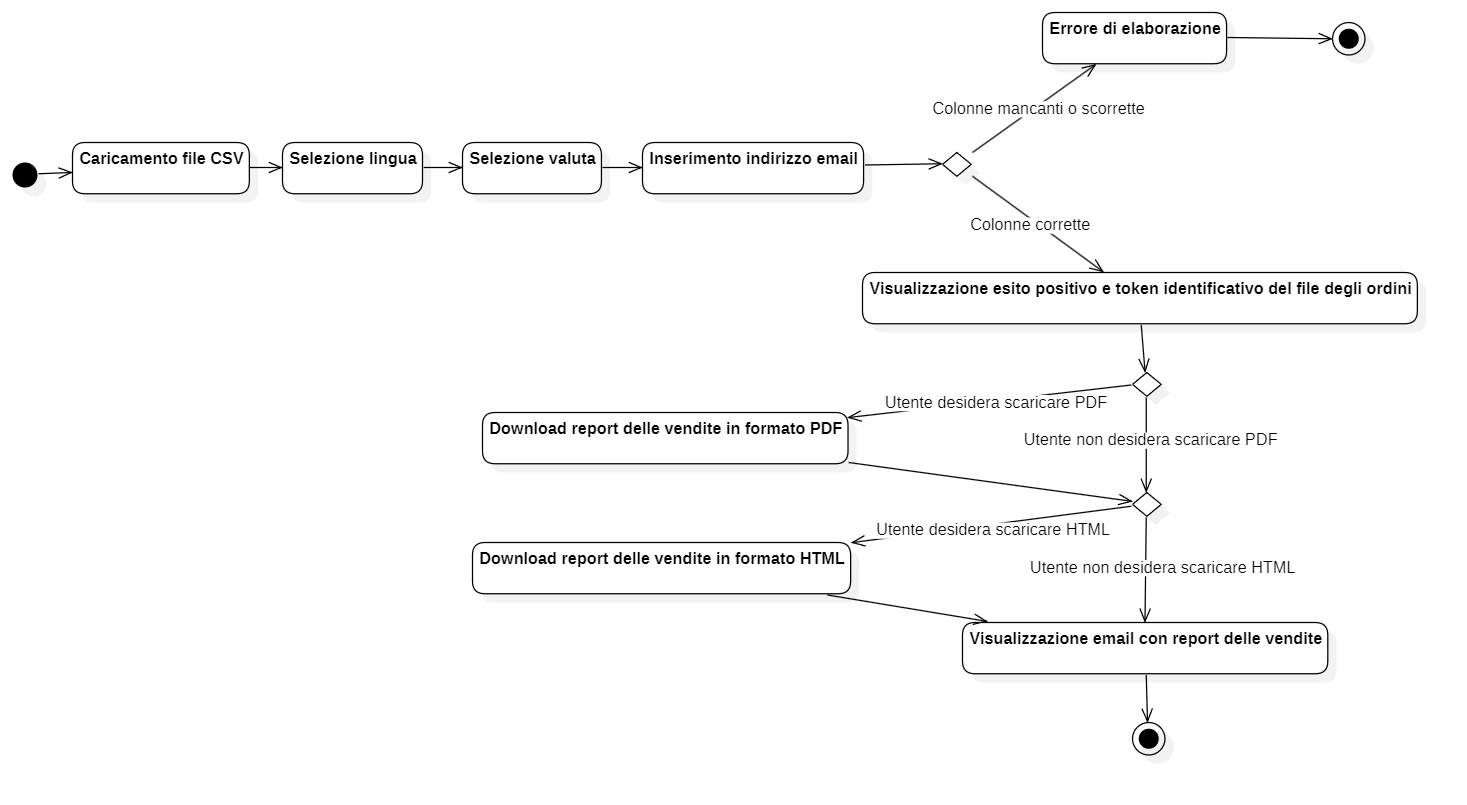
\includegraphics[width=0.9\columnwidth]{activity/Task di analisi delle vendite.png}
    \caption{Flusso delle attività della task di analisi delle vendite}
    \label{fig:activity-sales-analysis}
\end{figure}

Il flusso delle attività per la task di analisi delle vendite è rappresentato nella figura \ref{fig:activity-sales-analysis}. Le attività in sequenza previste dalla task dal lato dell'utente sono:
\begin{itemize}
    \item \textbf{Compilazione dei campi di input}: l'utente deve compilare i campi di input richiesti, cioè deve selezionare il file CSV contenente i dati delle vendite, selezionare la lingua del report e la valuta da utilizzare per i prezzi, e inserire l'indirizzo email a cui inviare il report;
    \item \textbf{Possibili output}: nel caso in cui l'utente abbia inserito correttamente i campi di input e nel caso la task non abbia riscontrato errori, l'utente visualizzerà un messaggio di esito positivo ed un invito a controllare la propria email per il report generato. Viene inoltre segnalata la generazione delle matrici di raccomandazione, e viene visualizzato il token che serve copiare per poter usufruire della task di raccomandazione. In caso la task non vada a buon fine, l'utente visualizzerà un messaggio di errore;
    \item \textbf{I file generati}: la task genera un file PDF ed un file HTML contenenti il report delle vendite, e l'utente ha la possibilità di scaricarli dall'apposita schermata del portale Oribea;
    \item \textbf{La ricezione della mail}: l'utente riceve una mail all'indirizzo email inserito in precedenza, il cui body contiene l'HTML del report, e riporta come allegati il report delle vendite in formato PDF ed HTML; inoltre, viene mostrato anche qui il token che serve copiare per poter usufruire della task di raccomandazione.
\end{itemize}

\begin{figure}[!h]
    \centering 
    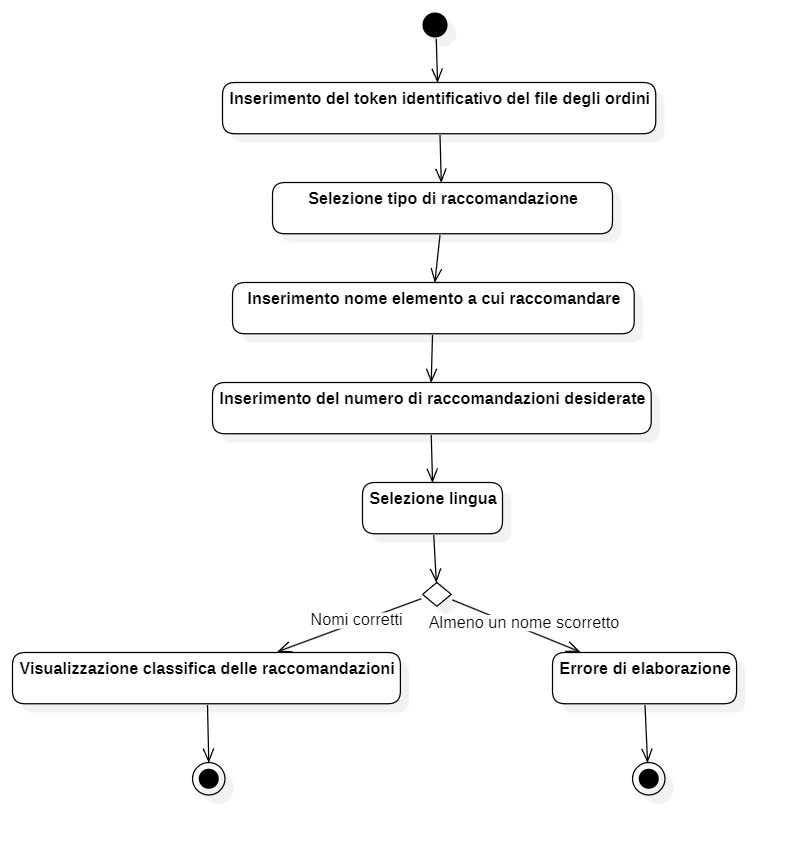
\includegraphics[width=0.9\columnwidth]{activity/Task di raccomandazione di prodotti e clienti.png}
    \caption{Flusso delle attività della task di raccomandazione di prodotti e clienti}
    \label{fig:activity-recommendation-products-customers}
\end{figure}

Il flusso delle attività per la task di raccomandazione di prodotti e clienti è rappresentato nella figura \ref{fig:activity-recommendation-products-customers}. Le attività in sequenza previste dalla task dal lato dell'utente sono:
\begin{itemize}
    \item \textbf{Compilazione dei campi di input}: l'utente deve compilare i campi di input richiesti, cioè deve inserire il token ricevuto nella mail della task di analisi delle vendite, selezionare il tipo di raccomandazione tra "Raccomandare prodotti per un cliente" e "Raccomandare clienti per un prodotto", inserire il nome dell'elemento a cui raccomandare, inserire il numero di raccomandazioni desiderate, e selezionare la lingua con cui presentare la classifica di raccomandazioni;
    \item \textbf{Possibili output}: nel caso in cui l'utente abbia inserito correttamente i campi di input e nel caso la task non abbia riscontrato errori, l'utente visualizzerà la classifica di raccomandazioni generata. In caso la task non vada a buon fine, l'utente visualizzerà un messaggio di errore.
\end{itemize}


\section{Tecnologie e strumenti}
\label{sec:tecnologie-strumenti}

Di seguito viene data una panoramica delle tecnologie e strumenti utilizzati per lo sviluppo delle due task di analisi delle vendite e raccomandazione di prodotti e clienti. Le tecnologie sono state scelte in base alle esigenze del progetto, alla facilità d'uso e alla compatibilità con le altre componenti del sistema.

\subsection{Pandas}
Pandas è una libreria Python per l'analisi dei dati, che fornisce strutture dati e funzioni per la manipolazione e l'analisi dei dati. È stata utilizzata per leggere i file CSV contenenti i dati delle vendite e per elaborare i dati in fase di preprocessing.

\subsection{Babel}
Babel è una libreria Python per la gestione della localizzazione e internazionalizzazione delle applicazioni. È stata utilizzata per gestire le date nel report, in modo da poterle visualizzare nel formato corretto in base alla lingua selezionata dall'utente.

\subsection{Anthropic}
Anthropic è una libreria che consente di interagire con i modelli di linguaggio di grandi dimensioni (\gls{llm}) sviluppati dall'azienda Anthropic tramite le loro API. In particolare, è stato usato il modello Claude 3.7 Sonnet per riconoscere le colonne del file CSV contenente i dati delle vendite, e per generare il resoconto finale che fa da ultimo passaggio del report delle vendite.

\subsection{Matplotlib}
Matplotlib è una libreria Python per la creazione di grafici e visualizzazioni dei dati. È stata utilizzata per generare i grafici presenti nel report delle vendite, in modo da rendere i dati più comprensibili e visivamente accattivanti.

\subsection{Pillow}
Pillow è una libreria Python per la manipolazione delle immagini. È stata utilizzata per generare le immagini dei grafici creati con Matplotlib e per la loro conversione in base64, in modo da poterli inserire nel report delle vendite in formato PDF ed HTML.

\subsection{ReportLab}
ReportLab è una libreria Python per la generazione di documenti PDF, che fornisce una disposizione dinamica del contenuto in pagine. È stata utilizzata per creare il report delle vendite in formato PDF, in modo da renderlo scaricabile dal portale Oribea e da poterlo inviare via email all'utente.

\subsection{Jinja2}
Jinja2 è un motore di template per Python, che consente di generare documenti HTML in modo dinamico. È stata utilizzata per creare il report delle vendite in formato HTML, in modo da renderlo visualizzabile direttamente nel browser e da poterlo anche inviare via email all'utente.

\subsection{Server SMTP interno}
Per l'invio di email, è stato utilizzato un server SMTP messo a disposizione da Oribea, che consente di inviare mail personalizzate senza avere la necessità di utilizzare un indirizzo mail esistente o di collegarsi ad un servizio esterno a pagamento. 

\subsection{Sentence Transformers}
SentenceTransformers è una libreria Python per la creazione di modelli di linguaggio basati su trasformatori, che consente di generare rappresentazioni vettoriali di frasi e documenti. È stata utilizzata per calcolare le similarità tra le descrizioni dei prodotti e i nomi dei prodotti, in modo da poter generare le raccomandazioni. In particolare, è stato utilizzato il modello \emph{all-MiniLM-L6-v2} per generare le rappresentazioni vettoriali delle descrizioni dei prodotti e dei nomi dei prodotti, e per calcolare la similarità tra di essi.

\subsection{Scikit-learn}
Scikit-learn è una libreria Python per il machine learning, che fornisce strumenti per la creazione e l'addestramento di modelli di apprendimento automatico. È stata utilizzata per calcolare la similarità tra le descrizioni dei prodotti e i nomi dei prodotti, in modo da poter generare le raccomandazioni. In particolare, è stato utilizzato il metodo \emph{cosine similarity} per calcolare la similarità tra i vettori delle descrizioni dei prodotti e i vettori dei nomi dei prodotti.

\subsection{Zarr}
Zarr è una libreria Python per la gestione di array multidimensionali, che consente di memorizzare e gestire grandi quantità di dati in modo efficiente. È stata utilizzata per memorizzare su cloud le matrici di raccomandazione generate dalla prima task, in modo da poterle utilizzare successivamente per le raccomandazioni nella seconda task.

\subsection{Google Cloud Storage}
Google Cloud Storage è un servizio di archiviazione di oggetti su cloud fornito da Google. È stato utilizzato per memorizzare i file generati dalla task di analisi delle vendite, come il report in formato PDF ed HTML, e le matrici di raccomandazione generate dalla task di raccomandazione di prodotti e clienti. In particolare, sono stati utilizzati i pacchetti \emph{google.cloud.storage} e \emph{gcsfs} per interagire con il servizio: \emph{google.cloud.storage} è stato utilizzato per scrivere i file, mentre \emph{gcsfs} è stato utilizzato per leggerli.

\subsection{Google Cloud Functions}
Google Cloud Functions è un servizio di calcolo serverless fornito da Google, che consente di eseguire codice in risposta a eventi. È stato utilizzato per caricarvi il codice delle due task di analisi delle vendite e raccomandazione di prodotti e clienti, in modo da poterle eseguire in modo scalabile e senza doversi preoccupare della gestione dei server. Il portale Oribea è configurato per invocare le funzioni di Google Cloud Functions quando l'utente richiede l'esecuzione delle task.

\subsection{Numpy}
Numpy è una libreria Python per il calcolo scientifico, che fornisce strutture dati e funzioni per la manipolazione di array multidimensionali. È stata utilizzata per calcolare le metriche di valutazione delle raccomandazioni.

\subsection{Black}
Black è un formattatore di codice Python che consente di mantenere uno stile di codifica coerente e leggibile. È stato utilizzato per formattare il codice delle due task, in modo da renderlo più leggibile e mantenere uno stile di codifica uniforme.

\subsection{Ruff}
Ruff è un linter per Python che consente di rilevare errori di sintassi e problemi di stile nel codice. È stato utilizzato per verificare la correttezza del codice delle due task, in modo da garantire che fosse privo di errori e conforme agli standard di codifica.

\subsection{MyPy}
MyPy è un tipo di controllo per Python che consente di verificare la correttezza dei tipi di dati nel codice. È stato utilizzato per verificare la correttezza dei tipi di dati delle due task, in modo da garantire che il codice fosse privo di errori di tipo e conforme agli standard di codifica.

\subsection{Pytest}
Pytest è un framework di testing per Python che consente di scrivere e eseguire test automatizzati. È stato utilizzato per testare le due task, in modo da garantire che funzionassero correttamente e fossero prive di errori. I test sono stati scritti in modo da coprire i casi d'uso principali delle due task, e sono stati eseguiti automaticamente durante lo sviluppo per garantire la qualità del codice.


\section{Architettura del sistema}

Prima di cominciare a sviluppare le due task, è stata svolta un'analisi preliminare per definire l'architettura del sistema e le interazioni tra le varie componenti. Siccome le task rappresentano due funzionalità distinte, è stato deciso di svilupparle come due funzioni separate su Google Cloud Functions, e quindi come due diversi progetti il più separati possibile, in modo da poterle gestire in modo indipendente e poterle testare separatamente.
Per entrambi i progetti, è stato deciso di utilizzare il linguaggio Python, in modo da poter sfruttare le librerie e gli strumenti già descritti nella sezione \ref{sec:tecnologie-strumenti}.
Inoltre, per entrambi è stato scelto un approccio procedurale a discapito di un approccio orientato agli oggetti, poiché le task sono relativamente semplici e non richiedono una struttura complessa. Tuttavia, è stato deciso di utilizzare i moduli Python per organizzare il codice in modo modulare e rendere più facile la lettura e la manutenzione del codice.
I moduli Python sono rappresentati da cartelle e da file con estensione \emph{.py}, e sono stati utilizzati per raggruppare le funzioni correlate e per separare le responsabilità del codice. In particolare, sono stati creati i moduli descritti di seguito.

Per quanto riguarda la task di analisi delle vendite, sono stati creati i seguenti moduli:
\begin{itemize}
    \item \textbf{preparation}: questo modulo, rappresentato da una cartella, contiene tutti i file necessari per l'inizializzazione del sistema e per l'elaborazione dei dati prima dell'analisi delle vendite. In particolare, contiene i seguenti sottomoduli:
    \begin{itemize}
        \item \textbf{Dependency Injection}: questo modulo, rappresentato da un file \emph{.py}, contiene le funzioni per l'iniezione delle dipendenze necessarie per l'esecuzione della task, come i parametri di configurazione delle API verso l'\gls{llm}\glsfirstoccur{} Anthropic e verso il server SMTP interno di Oribea;
        \item \textbf{Preprocessing}: questo modulo, rappresentato da un file \emph{.py}, contiene le funzioni per il preprocessing dei dati delle vendite, in particolare la funzione che va a chiamare l'\gls{llm} Anthropic per riconoscere le colonne del file CSV contenente i dati delle vendite e le funzioni di standardizzazione dei nomi e di sanificazione dei dati;
        \item \textbf{Language Processing}: questo modulo, rappresentato da un file \emph{.py}, contiene le funzioni per il processamento del linguaggio naturale, in particolare le funzioni per la formattazione delle date e per la selezione dei testi corretti in base alla lingua selezionata dall'utente.
    \end{itemize}
    \item \textbf{report}: questo modulo, rappresentato da una cartella, contiene tutti i file necessari per la generazione del report delle vendite. In particolare, contiene i seguenti sottomoduli:
    \begin{itemize}
        \item \textbf{calculations\_charts}: questo modulo, rappresentato da un file \emph{.py}, contiene le funzioni per il calcolo delle statistiche e dei trend di vendita e per la generazione dei grafici da inserire nel report delle vendite;
        \item \textbf{generate\_report}: questo modulo, rappresentato da un file \emph{.py}, contiene le funzioni per la generazione del report delle vendite in formato PDF ed HTML, utilizzando le librerie ReportLab e Jinja2. Contiene inoltre le funzioni di supporto per la generazione del report, come la funzione di conversione delle immagini dei grafici in base64, la funzione per chiedere all'\gls{llm} Anthropic di generare il resoconto finale del report, e le funzioni per la conversione della risposta ottenuta dall'\gls{llm} da Markdown a flowables (per il PDF) e a HTML;
        \item \tetxbf{send\_email}: questo modulo, rappresentato da un file \emph{.py}, contiene la funzione per l'invio dell'email all'utente con il report delle vendite in formato PDF ed HTML, che utilizza il server SMTP interno di Oribea, e una funzione di supporto per la creazione del body della mail.
    \end{itemize}
    \item \textbf{matrices}: questo modulo, rappresentato da un file \emph{.py}, contiene le funzioni per la generazione delle matrici di raccomandazione, che vengono salvate in oggetti di tipo Zarr. In particolare, contiene le funzioni per la generazione delle matrici di raccomandazione dei prodotti e dei clienti;
    \item \textbf{main}: questo modulo, rappresentato da un file \emph{.py}, contiene la funzione principale che viene eseguita quando la task viene invocata, e che coordina l'esecuzione delle altre funzioni dei moduli scritti in precedenza. Inoltre, contiene le funzioni per l'upload in Google Cloud Storage dei file generati dalla task, come il report delle vendite in formato PDF ed HTML e le matrici di raccomandazione.
\end{itemize}

Per quanto riguarda la task di raccomandazione di prodotti e clienti, sono stati creati i seguenti moduli:
\begin{itemize}
    \item \textbf{prediction}: questo modulo, rappresentato da una cartella, contiene tutti i file necessari per la predizione delle raccomandazioni. In particolare, contiene i seguenti sottomoduli:
    \begin{itemize}
        \item \textbf{predictor}: questo modulo, rappresentato da un file \emph{.py}, contiene le funzioni dirette per la predizione delle raccomandazioni, che utilizzano le matrici di raccomandazione generate dalla task di analisi delle vendite. Esso contiene anche l'algoritmo di rank fusion, che combina assieme le raccomandazioni ottenute dalle matrici;
        \item \textbf{filter}: questo modulo, rappresentato da un file \emph{.py}, contiene le funzioni per il filtraggio delle raccomandazioni, in modo da rimuovere, a seconda del caso, i prodotti già acquistati dall'utente ricevuto in input oppure gli utenti che hanno già acquistato il prodotto ricevuto in input;
        \item \textbf{make\_prediction}: questo modulo, rappresentato da un file \emph{.py}, contiene le funzioni per la creazione della predizione delle raccomandazioni, che utilizzano le funzioni dei moduli \emph{predictor} e \emph{filter} per generare la classifica di raccomandazioni. Contiene inoltre una funzione di explanation che stampa su console i passaggi intermedi della predizione, per facilitare il debug e la comprensione del funzionamento della task;
        \item \textbf{build\_output}: questo modulo, rappresentato da un file \emph{.py}, contiene una funzione che costruisce l'output della task, cioè inserisce un'introduzione ed una conclusione, selezionate in base alla lingua scelta dall'utente, attorno alla classifica di raccomandazioni.
    \end{itemize}
    \item \textbf{evaluation}: questo modulo, rappresentato da una cartella, contiene tutti i file necessari per la valutazione delle raccomandazioni. In particolare, contiene i seguenti sottomoduli:
    \begin{itemize}
        \item \textbf{metrics}: questo modulo, rappresentato da un file \emph{.py}, contiene le funzioni per il calcolo delle metriche di valutazione delle raccomandazioni. Queste metriche vengono calcolate confrontando le raccomandazioni generate dalla task con le vendite passate dei prodotti o dei clienti;
        \item \textbf{check\_metrics}: questo modulo, rappresentato da un file \emph{.py}, contiene le funzioni per il controllo delle metriche di valutazione delle raccomandazioni, in modo da verificare se le raccomandazioni generate sono valide e soddisfacenti. In particolare, vengono richiamate le funzioni del modulo \emph{metrics} per calcolare le metriche di valutazione, che vengono stampate su console, assieme al loro significato, per facilitare il debug e la comprensione del funzionamento della task.
    \end{itemize}
    \item \textbf{main}: questo modulo, rappresentato da un file \emph{.py}, contiene la funzione principale che viene eseguita quando la task viene invocata, e che coordina l'esecuzione delle altre funzioni dei moduli scritti in precedenza. Inizialmente, essa si occupa di cercare in Google Cloud Storage il bucket identificato dal token ricevuto in input, e di caricare le matrici di raccomandazione da esso. Successivamente, essa richiama le funzioni del modulo \emph{prediction/make\_prediction} per generare la classifica di raccomandazioni, e quelle del modulo \emph{evaluation/check\_metrics} per calcolare le metriche di valutazione delle raccomandazioni. Infine, essa restituisce l'output della task, cioè la classifica di raccomandazioni.
\end{itemize}

Sono stati appena descritti i moduli contenuti dentro la cartella \emph{src} di ciascuna task, che rappresentano il cuore del codice dei due progetti. Attorno a tale cartella, è stata creata una struttura di cartelle e file che rappresentano la configurazione del progetto, le dipendenze necessarie per l'esecuzione delle task, i test automatizzati e un file main per collegarsi al servizio Cloud Functions. In particolare, sono stati creati i seguenti file e cartelle:
\begin{itemize}
    \item \textbf{requirements.txt}: questo file contiene le dipendenze necessarie per l'esecuzione delle task, che vengono installate automaticamente quando si carica il codice su Google Cloud Functions;
    \item \textbf{.gcloudignore}: questo file contiene le regole per ignorare i file e le cartelle che non devono essere caricati su Google Cloud Functions, come i file di test e i file di configurazione locali;
    \item \textbf{tests}: questa cartella contiene i test automatizzati per le due task, che vengono eseguiti automaticamente durante lo sviluppo per garantire la qualità del codice. I test sono scritti utilizzando il framework Pytest, e sono organizzati in moduli separati per ciascuna task;
    \item \textbf{main.py}: questo file contiene il codice principale per collegarsi al servizio Cloud Functions, e richiama la funzione principale della task corrispondente;
    \item \textbf{pyproject.toml}: questo file contiene la configurazione del progetto, come il nome del progetto, la versione, la descrizione e le dipendenze necessarie per l'esecuzione delle task. Inoltre, contiene le configurazioni per i tool di formattazione e linting del codice, come Black, Ruff e MyPy;
    \item \textbf{pytest.ini}: questo file contiene la configurazione per Pytest, il framework di testing utilizzato per i test automatizzati delle due task. In particolare, contiene la configurazione della coverage a 75\% per i test, e la configurazione per eseguire i test per l'\gls{llm} separatamente rispetto ai test "classici";
    \item \textbf{file .bat}: script per l'esecuzione dell'analisi statica del codice, che eseguono i tool di formattazione e linting Black, Ruff e MyPy. Questi script sono stati creati per facilitare l'esecuzione di questi ultimi tool, in modo da poterli consultare facilmente durante lo sviluppo.
\end{itemize}



\section{Preprocessing}
\label{sec:preprocessing}

\subsection{Riconoscimento delle marche}
\label{sec:recognition-brands}

Per poter analizzare le vendite in modo più dettagliato, è stato pensato di introdurre una colonna "Marca" nei dataset, che potesse contenere il nome della marca del prodotto presente in tale riga. Per ottenere ciò, era dunque necessario sviluppare un sistema di riconoscimento delle marche. Sono state provate le seguenti strategie:
\begin{itemize}
    \item \textbf{Riconoscimento tramite dizionario}: è stato creato un dizionario contenente le marche più comuni, ma si è rivelato poco efficace, poiché molte marche non erano presenti nel dizionario e il riconoscimento era limitato;
    \item \textbf{Riconoscimento tramite regex}: è stato provato a utilizzare delle espressioni regolari per riconoscere le marche, ma si è rivelato poco efficace, poiché molte marche non seguivano uno schema comune e il riconoscimento era limitato;
    \item \textbf{Riconoscimento tramite modelli di \gls{ml}\glsfirstoccur{}}: è stato pensato di creare un modello di \gls{ml} per riconoscere le marche, ma si è rivelato poco efficace, poiché il dataset non era sufficientemente grande e vario per addestrare un modello affidabile, e soprattuto non erano disponibili le etichette necessarie per un addestramento supervisionato;
    \item \textbf{Riconoscimento tramite modelli di \gls{ner}\glsfirstoccur{}}: è stato provato ad utilizzare un modello di \gls{ner} sulle descrizioni dei prodotti e a selezionare le entità segnalate di tipo \emph{ORG} (organizzazione), ma si è rivelato poco efficace, poiché il modello non era stato addestrato specificamente per questo compito e il riconoscimento era limitato;
    \item \textbf{Riconoscimento tramite \gls{llm}\glsfirstoccur{}}: è stato provato ad utilizzare un modello di linguaggio di grandi dimensioni (\gls{llm}) per riconoscere le marche, e si è rivelato mediamente efficace, ma il riconoscimento di ciascuna marca richiedeva troppo tempo e tantissime chiamate \gls{api}\glsfirstoccur{}; allora, è stato fatto un tentativo di raggruppamento di più descrizioni da inviare assieme per il riconoscimento di più marche contemporaneamente, ma si è rivelato poco efficace, poiché il modello ogni tanto si dimenticava di alcune marche o ne aggiungeva qualcuna in più, totalmente senza motivo (avvenivano cioè le cosidette "allucinazioni").
\end{itemize}

Dunque, si è deciso di non implementare il riconoscimento delle marche nel sistema di analisi automatizzato, poiché non era possibile garantire un riconoscimento affidabile e preciso.


\subsection{Riconoscimento delle categorie}
\label{sec:recognition-categories}

Per poter analizzare le vendite in modo più dettagliato, è stato pensato di introdurre una colonna "Categoria" nei dataset, che potesse contenere il nome della categoria del prodotto presente in tale riga. Per ottenere ciò, era dunque necessario sviluppare un sistema di riconoscimento delle categorie.

Escluse le opzioni già descritte nella sezione \ref{sec:recognition-brands} per il riconoscimento delle marche, è stato pensato di utilizzare un modello \gls{kmeans}\glsfirstoccur{} per raggruppare i prodotti in base alle loro descrizioni, in modo da ottenere delle categorie. Tuttavia, ciò si è rivelato poco efficace, poiché il modello non era in grado di raggruppare i prodotti in categorie in modo affidabile e preciso, e il numero di categorie era troppo elevato per poterle gestire manualmente.

Dunque, si è deciso di non implementare il riconoscimento delle categorie nel sistema di analisi automatizzato, poiché non era possibile garantire un riconoscimento affidabile e preciso.\\



\section{Language processing}
\label{sec:language-processing}

\section{Report}
\subsection{PDF}
\subsection{HTML}

\section{Invio di email}

\section{Le matrici di raccomandazione}

\subsection{Formato di archiviazione delle matrici}

Considerati l'elevato consumo di spazio e la lentezza di accesso ai dati delle matrici di raccomandazione salvate come file CSV, si è deciso di svolgere un'analisi preliminare per valutare il formato di archiviazione più adatto. Sono stati presi in considerazione i seguenti formati:
\begin{itemize}
    \item \textbf{CSV}: il formato CSV (Comma-Separated Values) è un formato di testo semplice e ampiamente utilizzato per la memorizzazione di dati tabellari. È stato preso in considerazione per la sua semplicità, portabilità e compatibilità con numerosi strumenti di analisi dati;
    \item \textbf{HDF5}: HDF5 (Hierarchical Data Format version 5) è un formato binario progettato per la gestione efficiente di grandi quantità di dati complessi e strutturati. È stato valutato per le sue capacità di compressione, accesso rapido e supporto a dataset multidimensionali;
    \item \textbf{NPY}: il formato NPY è il formato binario nativo di NumPy per la memorizzazione di array multidimensionali. È stato considerato per la sua efficienza nello storage e nella lettura di array numerici in ambiente Python;
    \item \textbf{Parquet}: Parquet è un formato di archiviazione colonnare ottimizzato per l'analisi di grandi volumi di dati. È stato preso in considerazione per le sue prestazioni elevate, la compressione e la compatibilità con diversi framework di big data;
    \item \textbf{Zarr}: Zarr è un formato per la memorizzazione di array multidimensionali che supporta la compressione e l'accesso parallelo ai dati. È stato valutato per la sua scalabilità, flessibilità e facilità di integrazione con sistemi cloud.
\end{itemize}

Sono stati dunque sviluppati dei test automatizzati per confrontare le prestazioni di lettura dei vari formati e lo spazio occupato su disco. I tempi di scrittura non sono stati considerati, poiché le matrici di raccomandazione vengono generate una sola volta e poi salvate su Google Cloud Storage, dove rimangono per essere utilizzate in seguito. I dataset che sono stati utilizzati per i test sono stati scelti cercando di variare la dimensione e la densità delle matrici, e sono qui di seguito elencati in ordine crescente di dimensione:
\begin{table}[h]
    \centering
    \begin{tabular}{|l|c|}
        \hline
        \textbf{Dataset} & \textbf{Dimensioni della matrice} \\
        \hline
        Feroze & 10 $\times$ 10 \\
        Vaghasiya & 2.172 $\times$ 268 \\
        Anwer & 795 $\times$ 10.292 \\
        Delikkaya & 35.389 $\times$ 1.000 \\
        Orders\_export & 23.389 $\times$ 4.114 \\
        Cornelius & 14.095 $\times$ 15.000 \\
        \hline
    \end{tabular}
    \caption{Dataset utilizzati per il confronto dei formati di archiviazione delle matrici di raccomandazione}
    \label{tab:dataset-matrici}
\end{table}


\section{La predizione e rank fusion}

\section{Valutazione delle raccomandazioni}

\section{Collegamento con Google Cloud}
\subsection{Google Cloud Storage}
\subsection{Google Cloud Functions}
